\documentclass[11pt]{article}

%\pagestyle{empty}

\hyphenation{con-si-de-ra-to}

%\textwidth=182mm
%\textheight=230mm
%\hoffset=-31mm                  % horizontal offset
%\voffset=-30mm                  % vertical offset

\usepackage[margin=.775in]{geometry}

\usepackage[usenames]{color}
%\usepackage[mathcal]{eucal}
\usepackage{epsfig}
\usepackage{amsmath}
\usepackage{amssymb}
\usepackage{amsthm}
\usepackage{amsfonts}
\usepackage{enumerate}
\usepackage{amsthm}
\usepackage{dsfont}
\usepackage[usenames]{color}
\usepackage{wrapfig}
\usepackage{graphicx}
\usepackage{blindtext}
\usepackage{enumerate}
\usepackage{fancyvrb}
\usepackage{esint}

\usepackage{listings}
\usepackage{color}
 
\definecolor{codegreen}{rgb}{0,0.6,0}
\definecolor{codegray}{rgb}{0.5,0.5,0.5}
\definecolor{codepurple}{rgb}{0.58,0,0.82}
\definecolor{backcolour}{rgb}{0.95,0.95,0.92}
 
\lstdefinestyle{mystyle}{
    backgroundcolor=\color{backcolour},   
    commentstyle=\color{codegreen},
    keywordstyle=\color{magenta},
    numberstyle=\tiny\color{codegray},
    stringstyle=\color{codepurple},
    basicstyle=\footnotesize,
    breakatwhitespace=false,         
    breaklines=true,                 
    captionpos=b,                    
    keepspaces=true,                 
    numbers=left,                    
    numbersep=5pt,                  
    showspaces=false,                
    showstringspaces=false,
    showtabs=false,                  
    tabsize=2
}
 
\lstset{style=mystyle}

\usepackage{lscape}

\usepackage{color,hyperref}
\definecolor{darkblue}{rgb}{0.0,0.0,.45}
\definecolor{darkred}{rgb}{0.7,0,0}
\hypersetup{colorlinks,breaklinks,
	linkcolor=darkred,urlcolor=darkred,
	anchorcolor=darkred}


\newcommand{\myparallel}{{\mkern3mu\vphantom{\perp}\vrule depth 0pt\mkern2mu\vrule depth 0pt\mkern3mu}}

\newcommand{\qq}{\mathbf{q}}
\newcommand{\qqd}{\mathbf{\dot{q}}}
\newcommand{\ind}{\mathds{1}} % so $\ind{1}$ gives you the script 1
\newcommand{\gul}[2]{g^{#1 ,}_{\textcolor{White}{#1}#2\ }}

\theoremstyle{plain}
\newtheorem{corollary}{Corollary}
\newtheorem{proposition}{Proposition}
\newtheorem{lemma}{Lemma}
\theoremstyle{definition}
\newtheorem{definition}{Definition}
\newtheorem{example}{Example}
\newtheorem{case}{Case}
\newtheorem{conj}{Conjecture}
\newtheorem*{remark}{Remark}
\newtheorem*{notation}{Notation}
%\newtheorem{fc1}{From Chapter 1 of Millman \& Parker:}
%\newtheorem{fc2}{From Chapter 1 of Millman \& Parker:}
\newtheorem{problem}{Problem}
\newtheorem{theorem}{Theorem}
\newtheorem{solution}{Solution}
%\renewcommand*{\theproblem}{\hwn\Alph{problem}}
\renewcommand*{\theproblem}{\hwn.\arabic{problem}}
\renewcommand*{\thesolution}{\hwn.\arabic{solution}}
%\newtheorem{theorem}{Theorem}
\theoremstyle{remark}

\parindent=0cm



\newcommand{\hwn}{3}

\newcommand{\compconj}[1]{%
  \overline{#1}%
}


\begin{document}
\LARGE
\noindent{\textsf{\textbf{CGU Math 381 (Image Processing), Spring '18 
			-- Homework \#\hwn}}}
\par\vspace{.25cm}
\Large
\hspace{.5cm}\textsf{\mbox{%
Corner deteection, and an introduction to Fourier Analysis. 
}}
\par\vspace{.2cm}
\normalsize
\hspace{.5cm}\mbox{\textsf{\em Due 
		on Friday 3/30, in the box in front of Prof.~Micheli's office. }%
}

\hspace{.5cm}\mbox{\textsf{\em Song, Zhengming, Claremont Graduate University}
}
\par\vspace{.3cm}
\normalsize\rm
%$\boxed{\mbox{ \bf This homework assignment is on two
%		 pages. }}$ \par\vspace{.3cm}
\bf Reading: \rm
Fourier Analysis is treated in Chapters 7, 8 and 9 of 
\em Principles of Digital Image
Processing: Core Algorithms \em (i.e.~Volume 2) by Burger and Burge.
The Harris corner detector is treated Chapter 4
of the same volume, and (in more detail) in the instructor's class 
notes, that are now available online.
\par\vspace{.15cm}
Write, on top of the first page of your assignment:
Name (\underline{LAST}, First), your University or College, the HW\#, and acknowledge other students
with whom you may have worked (just write \mbox{``\em Worked with \ldots\/\em''}). For the computational problems 
where you are asked to write computer code you may choose 
the programming language that you prefer, such as \em Python \em 
(I am learning it myself!) or
\em Matlab\em\/.
%\par\vspace{.15cm}
%Solve the following problems:
%\par\vspace{.15cm}
%In the problems that follow, we shall employ the following notation:
%\begin{align*}
%b & =\mbox{\# of bits per pixel (typically $b=8$),}
%&
%L & =2^b =\mbox{\# of gray levels,}
%&
%\mathbb{P} & =\{0,1,2,\ldots,L-1\},
%\\ 
%\mathbb{D} & =\{0,1,\ldots,M-1\}\times
%\{0,1,\ldots,N-1\}, \mbox{ where:}
%&
%M & =\mbox{\# rows},
%&
%N & =\mbox{\# columns}.
%\end{align*}
\begin{problem}[time shifting]
Consider the \em shifted \em delta function
$\delta_{t_0}(t)=\delta(t-t_0)$. {\bf(a)}~Show that
for any continuous-time signal~$s(t)$, $t\in \mathbb{R}$,
it is the case that~$(s\ast\delta_{t_0})(t)=s(t-t_0)$
(that is, the convolution with $\delta_{t_0}$ hs the effect
of time-shifting by~$t_0$). {\bf(b)}~find the 
Fourier Transform $\mathcal{F}[\delta_{t_0}](f)$
by direct computation.  
{\bf(c)}~Finally, 
combine the above results with the convolution theorem
(it states that~$\mathcal{F}[g\ast h](f)=G(f)H(f)$)
to find the Fourier Transform of the shifted signal~$s(t-t_0)$
in terms of the Fourier Transform~$S(f)$ of~$s(t)$.
\end{problem}
\begin{solution}
	\begin{enumerate}
		\item[a] 	
		\begin{eqnarray*}
			(s*\delta_{t_0})(t) = & \int_{-\infty}^{+\infty} s(\tau) \delta_{t_0} (t-\tau) d\tau\\
			= & \int_{-\infty}^{+\infty} s(\tau) \delta (t- t_0 -\tau) d\tau\\
			= & \int_{-\infty}^{+\infty} s(t-t_0) \delta(t-t_0 -\tau) d\tau \\
			= & s(t-t_0) \int_{-\infty}^{+\infty} \delta (t-t_0 -\tau) d\tau \\
			= & s(t-t_0) \int_{-\infty}^{+\infty} \delta (\tau - (t-t_0)) d\tau \\
			= & s(t-t_0) \cdot 1 \\
			= & s(t-t_0)
		\end{eqnarray*}
		
		\item[b]
		\begin{eqnarray*}
		\mathcal{F}[\delta t_0] (f) = & \int_{-\infty}^{+\infty} \delta_{t_0} (\tau) e^{-i 2\pi f \tau} d\tau\\
			= & \int_{-\infty}^{+\infty} \delta (\tau - t_0) e^{-i2\pi f \tau} d\tau\\
			 \overset{\mathrm{t = \tau - t_0}}{=} & \int_{-\infty}^{+\infty} \delta (t) e^{-i 2\pi f(t+t_0)} dt\\
			= & e^{-i2\pi t_0} \int_{-\infty}^{+\infty}  \delta (t) e^{-i2\pi ft}dt\\
			= &  e^{-i2\pi t_0} \cdot e^{-i2\pi f 0} \cdot \int_{-\infty}^{+\infty} \delta (t) dt\\
			= & e^{-i2\pi t_0}  \cdot 1 \cdot 1\\
			= & e^{-i2\pi t_0}
		\end{eqnarray*}
		
		\item[c]
		\begin{eqnarray*}
		\mathcal{F}[s(t-t_0)] (f) = & \mathcal{F}[s*\delta_{t_0}(t)](f) \\
		= & \mathcal{S}(f) \mathcal{D}(f)\\
		= & \mathcal{S}(f) \cdot \mathcal{F}[\delta_{t_0}](f) \\
		= & e^{-i2\pi f t_0} \mathcal{S}(f)
		\end{eqnarray*}
		
	\end{enumerate}

\end{solution}
\begin{problem}[the causal exponential]
Fix a constant~$\alpha>0$,
and consider the continuous-time 
signal
$s(t)=e^{-\alpha t}H(t)$, $t\in\mathbb{R}$,
known as the \em causal
exponential \em\/,
where $H(t)$ is the Heaviside function
(that is, $H(t)=1$ 
for $t\geq0$ and $H(t)=0$ for $t<0$).
{\bf(a)}~Compute its Fourier transform~$S(f)$, $f\in\mathbb{R}$
(this is example~\#26 in the Fourier pairs table that was 
distributed in class).
{\bf(b)}~Compute the convolution 
$r(t)=(s\ast s)(t)$, $t\in \mathbb{R}$
(this may be the first and last
time that you actually compute a convolution `by hand', but it iss the 
kind of thing that you should do at least 
once in your life!).
{\bf(c)}~Finally, using the result from part~{(a)},
what is the Fourier transform~$R(f)$ of the 
continuous-time signal~$r(t)$ from part~(b)? 
\end{problem}

\begin{solution}
	\begin{enumerate}
		\item[a]
		\begin{eqnarray*}
			\mathcal{S}(f) = & \mathcal{F} [s] (f) \\
			=& \int_{-\infty}^{+\infty} e^{-\alpha t} H(t) e^{-i2\pi ft} dt\\
			=& \int_{0}^{+\infty} e^{-\alpha t} e^{-i2\pi ft} dt\\
			=& \int_{0}^{+\infty} e^{-\alpha + i2\pi f}t dt\\	
			=& \frac{e^{-(\alpha + i 2 \pi f)t}}{-(\alpha + i 2\pi f)} |_{0}^{+\infty}\\
			=& 0 - \frac{-1}{\alpha + i2\pi f}\\
			=& \frac{1}{\alpha + i 2\pi f}
		\end{eqnarray*}
		\item[b]
		\begin{eqnarray*}
			r(t) =& (s*s)(t) \\
			=& \int_{-\infty}^{+\infty} s(\tau) s(t-\tau) d\tau\\
			=& \int_{-\infty}^{+\infty} e^{-\alpha \tau} H(\tau) e^{-\alpha(t-\tau)} H(t-\tau) d\tau\\
			=& e^{-\alpha t} \int_{-\infty}^{+\infty} H(\tau) H(t-\tau) d\tau\\
			=& e^{-\alpha t} t H(t)
		\end{eqnarray*}
		\item[c]
		\begin{equation*}
			\mathcal{R}(f) = \mathcal{F}[r](f) = \mathcal{S}\cdot \mathcal{S}(f) = \frac{1}{(\alpha + i 2\pi f) ^2}
		\end{equation*}
	\end{enumerate}
\end{solution}
\begin{problem}[FT of separable 2D signals]
Suppose that a signal $s(x,y)$, with $(x,y)\in\mathbb{R}^2$,
may be written as: $s(x,y)=f(x)g(y)$, where $f$ 
and $g$ are (continuous-space) signals. 
Such 2D signals are called \em separable\em\/.
Show that the Fourier transform of~$s$ is %given by
$S(u,v)=F(u)G(v)$, where~$F(u)=\mathcal{F}[f](u)$
and~$G(v)=\mathcal{F}[g](v)$. 
\end{problem}
\begin{solution}
	\begin{eqnarray*}
		\mathcal{S}(u,v) =& \int_{-\infty}^{+\infty} \int_{-\infty}^{+\infty}  s(x,y) e^{-i 2\pi (ux +vy)} dx dy\\
		=& \int_{-\infty}^{+\infty} \int_{-\infty}^{+\infty} f(x) g(y) e^{-i 2\pi (ux +vy)} dx dy\\
		=& \int_{-\infty}^{+\infty} g(y) e^{-i2\pi vy} \int_{-\infty}^{+\infty}  f(x) e^{-i2\pi ux} dxdy\\
		=& \int_{-\infty}^{+\infty} g(y) e^{-i2\pi vy} \mathcal{F}(u) dy\\
		=& \mathcal{F}(u) \int_{-\infty}^{+\infty}  \int_{-\infty}^{+\infty} g(y) e^{-i2\pi vy} dy\\
		=& \mathcal{F}(u) \mathcal{G}(v)
	\end{eqnarray*}
\end{solution}
\begin{problem}[differential operators and convolution]
Consider two continuous-space signals~$f(x,y)$ and~$g(x,y)$,
with $(x,y)\in\mathbb{R}^2$. {\bf(a)}~Show that
$\nabla^2(f\ast g)=f\ast(\nabla^2g)$, where $\nabla^2$
donotes the Laplace operator in the variables~$(x,y)$.
{\bf(b)}~Express the Fourier transform 
of~$\frac{\partial^2 f}{\partial x\partial y}$
in terms of~$F(u,v)=\mathcal{F}[f](u,v)$.
\end{problem}
\begin{solution}
	\begin{enumerate}
	\item[a]
	\begin{eqnarray*}
		\nabla^2 (f*g) (x,y) =& \nabla^2 \int_{-\infty}^{+\infty} \int_{-\infty}^{+\infty} f(u,v) g(x-u, y-v) dudv\\
		=& \int_{-\infty}^{+\infty}\int_{-\infty}^{+\infty} f(u,v) \cdot \nabla^2g(x-u,y-v)dudv\\
		=& (f*\nabla^2g)(x,y)
	\end{eqnarray*}
	
	\item[b]
	\begin{eqnarray*}
		\frac{\partial ^2 f}{\partial x\partial y} =& \frac{\partial}{\partial y}[\frac{\partial}{\partial x}(f)]\\
		=& \frac{\partial}{\partial y}[\frac{\partial}{\partial x}(\int_{-\infty}^{+\infty}\int_{-\infty}^{+\infty} F(u,v) e^{i2\pi (ux+vy)} dudv)]\\
		=&  \frac{\partial}{\partial y}[\int_{-\infty}^{+\infty}\int_{-\infty}^{+\infty} F(u,v) \frac{\partial}{\partial x} e^{i2\pi (ux+vy)} dudv]\\
		=& \frac{\partial}{\partial y}[\int_{-\infty}^{+\infty} i2\pi u \int_{-\infty}^{+\infty} F(u,v) e^{i2\pi (ux+vy)} dudv]\\
		=& [\int_{-\infty}^{+\infty} i2\pi u \int_{-\infty}^{+\infty} F(u,v) \frac{\partial}{\partial y} e^{i2\pi (ux+vy)} dudv]\\
		=& [\int_{-\infty}^{+\infty}  \int_{-\infty}^{+\infty} (i2\pi)^2 uvF(u,v) e^{i2\pi (ux+vy)} dudv]\\
	\end{eqnarray*}
	Hence,
	\begin{equation*}
	\mathcal{F}[\frac{\partial ^2 f}{\partial x\partial y}](u,v) = -4\pi^2 uv F(u,v)
	\end{equation*}
	\end{enumerate}
\end{solution}
\begin{problem}[symmetries]
Consider a continous-space signal~$s(x,y)$,
$(x,y)\in\mathbb{R}^2$. Show that if
the signal~$s$ is real and has even symmetry,
i.e.~$s(x,y)=\overline{s(x,y)}=\overline{s(-x,-y)}=s(-x,-y)$,
(where the bar indicates complex conjugation)
then its Fourier transform $S(u,v)$ is also real, with even symmetry.
\end{problem}
\begin{solution}
	\begin{eqnarray*}
		\mathcal{S}(u,v) =& \int_{-\infty}^{+\infty}  \int_{-\infty}^{+\infty} s(x,y) e^{-i 2\pi (ux +vy)} dxdy\\
		=& \int_{-\infty}^{+\infty}  \int_{-\infty}^{+\infty} s(x,y) [\cos(2\pi(ux+vy))-isin(2\pi(ux+vy)]dxdy\\
		=& \int_{-\infty}^{+\infty}  \int_{-\infty}^{+\infty} s(x,y) \cos(2\pi(ux+vy))dxdy + -i \int_{-\infty}^{+\infty}  \int_{-\infty}^{+\infty} s(x,y) \sin(2\pi(ux+vy))dxdy\\
		=& \int_{-\infty}^{+\infty}  \int_{-\infty}^{+\infty} s(x,y) \cos(2\pi(ux+vy))dxdy + 0\\
	\end{eqnarray*}
	The last equality hold because $\sin(\cdot)$ is a odd function, while $s(x,y)$ is a event function, hence, the product of those two functions are odd, and the integral of a odd function is $0$. In addition, since both $s(x,y)$ and $\cos(\cdot)$ are real, $\mathcal{S}(u,v)$ is real.
	
	\begin{eqnarray*}
		\mathcal{S}(-u, -v) = & \int_{-\infty}^{+\infty}  \int_{-\infty}^{+\infty} s(x,y) e^{i2\pi (-ux-vy)}dxdy \\
		\overset{\mathrm{x = -\alpha,  y = -\beta}}{=}  &  \int_{-\infty}^{+\infty}  \int_{-\infty}^{+\infty} s(x,y) e^{-i 2\pi (u\alpha + v\beta)} d\alpha d\beta \\
		=& \mathcal{S}(u,v)
	\end{eqnarray*}

\end{solution}
\begin{problem}[UMF in the  frequency domain]
Remember that the sharpening technique known as 
\em unmask filtering \em is defined as follows,
for continuous-space images $f(x,y)$.
First of all, a smoothing (low-pass) fiter, such as a 
Gaussian filter $h(x,y)=\frac{1}{2\pi\sigma^2}\exp\!
\big(\!-\!\frac{1}{2}\frac{x^2+y^2}{\sigma^2}\big)$
is chosen (note that since $h$ has volume~1, we have $H(0,0)=1$).
Then the smooth compunent of~$f$ is computed 
via convolution: $m=h\ast f$. The sharp component
of the image $f(x,y)$ (also known as the \em unsharp mask\em\/)
is $s(x,y)=f(x,y)-m(x,y)$. The sharpened image is then defined
as $g(x,y)=f(x,y)+a\cdot s(x,y)$, where the constant $a>0$ 
is the \em sharpening strentgh\em\/. For
a generic smoothing convolutional kernel~$h(x,y)$ with
Fourier transform~$H(u,v)$, show (as we did in class) 
that we can write, in frequency,~$G(u,v)=L(u,v)\cdot F(u,v)$;
express the frequency response~$L(u,v)$ in terms of the function~$H(u,v)$
and the constant~$a$. Also, write an explicit expression 
for~$L(u,v)$ when~$h(x,y)$ is the Gaussian function given above,
and plot the graph of~$z=L(u,v)$ for one or two particular choices of~$\sigma$ and~$a$ (since~$L(u,v)$ turns out to be a radial fucntion, i.e.~such that its graph is symmetric with respect
to rotations about the~$z$-axis, you may just plot the cross section for~$v=0$).
\end{problem}

\begin{solution}
	\begin{eqnarray*}
		g(x,y) = &f(x,y) + a\cdot s(x,y)\\
		=& f(x,y) + a\cdot f(x,y) - a\cdot h(x,y)*f(x,y)\\
	\end{eqnarray*}
	
	\begin{equation*}
			\mathcal{G}(u,v) = F(u,v) + a F(u,v) + a H(u,v)F(u,v) = (1+a+aH(u,v))F(u,v)
	\end{equation*}
	
	Hence,
	\begin{equation*}
	\mathcal{L}(u,v) =  (1+a+aH(u,v)) = (1+a-ae^{-2\pi \sigma^2(u^2+v^2)})
	\end{equation*}
	
	\begin{lstlisting}[language=Python, caption=Python Implementation of for Q6]
		import numpy as np
		import matplotlib.pyplot as plt
		%matplotlib inline
		from math import exp, pi
		a = 0.8
		sigma = 1
		u = np.linspace(start=-1, stop=1, dtype=np.float32)
		L = [1+a-a*exp(-2*pi*sigma**2*x**2) for x in u]
		fig = plt.figure(figsize=(8, 6))
		plt.plot(u,L)
		plt.show()
		fig.savefig('q6.png', dpi=fig.dpi)
	\end{lstlisting}
	
	\begin{figure}[h]
		\centering
		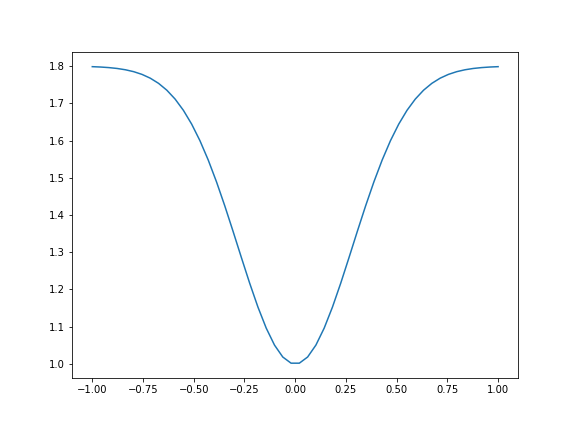
\includegraphics[width=\textwidth]{q6.png}
		\caption{$\mathcal{L}(u,v)$ with $v=0$}
	\end{figure}
	
\end{solution}
%\clearpage
\begin{problem}[DFT and IDFT]
In class we defined the Discrete Fourier Transform (DFT) of
a discrete- and finite-time signal~$s_n$, $n=0,1,\ldots, M-1$
as follows:
\par\vspace{.15cm}
\hfill
$
\displaystyle
S_k = 
\sum_{n=0}^{M-1}s_n\,e^{-i2\pi kn/M}
\qquad
k=0,1,\ldots, M-1.
$
\hfill\mbox{ }
\par\vspace{-.25cm}
Show that~$s_n$ can be recovered via
the Inverse Discrete Fourier Transform:
$\displaystyle
s_n=\frac{1}{M}
\sum_{k=0}^{M-1}S_k\,e^{+i2\pi kn/M}.
$
\par\vspace{.15cm}
{\em Hint:} You should first prove and then 
use the following \em orthogonality \em of
discrete complex exponentials:
\par\vspace{.15cm}
\hfill
$
\displaystyle
\sum_{k=0}^{M-1}
e^{i2\pi km/M}
e^{-i2\pi kn/M}=
\left\{
\begin{array}{ll}
M&\mbox{ if }m=n\\
0 &\mbox{ otherwise}.
\end{array}
\right.
$
\hfill\mbox{ }
\end{problem}
\begin{solution}
	First let's prove the orthogonality of discrete complex exponential:
	\begin{proof}
		\begin{equation*}
			\sum_{k=0}^{M-1} e^{i2\pi km/M}e^{-i2\pi kn/M} = \sum  e^{2\pi ki(m-n)/M}
		\end{equation*}
		if $m=n$, we have 
		$$ \sum  e^{2\pi ki(m-n)/M}= \sum 1 =M$$
		if $m\neq n$, we have
		\begin{eqnarray*}
			 \sum  e^{2\pi ki(m-n)/M} = & \sum [e^{\frac{2\pi i(m-n)}{M}}]^k\\
			 =& \frac{1-(e^{\frac{2\pi i (m-n)}{M}})^M}{1 - e^{\frac{2\pi i (m-n)}{M}}}
		\end{eqnarray*}
		Given that $m, n \in [0, 1, \cdots, M-1]$ hence, the denominator cannot be 0. however, in the numerator, 
		$$e^{2\pi i(m-n)} = \cos(2\pi(m-n)) + i\sin(2\pi(m-n)) = 1 + 0$$, which makes the numerator $0$.
		
		Hence, 
		$$
		\sum_{k=0}^{M-1}e^{i2\pi km/M}e^{-i2\pi kn/M} = \left\lbrace 
		\begin{array}{ll}
M&\mbox{ if }m=n\\
0 &\mbox{ otherwise}.
\end{array}
		\right.
		$$
	\end{proof}
	
	Next, we proof the main statement of this problem
	\begin{proof}
		\begin{eqnarray*}
			s_n =& \frac{1}{M} \sum	_{k=0}^{M-1} S_k e^{i2\pi kn/M}\\
			=&  \frac{1}{M} \sum	_{k=0}^{M-1} \sum_{m=0}^{M-1} s_m e^{-i 2\pi km/M} e^{i2\pi kn/M}\\
			=&  \frac{1}{M} \sum	_{m=0}^{M-1} s_m  \sum_{k=0}^{M-1}  e^{-i 2\pi km/M} e^{i2\pi kn/M}\\
			=& \frac{1}{M} \cdot s_n \cdot M\\
			=& s_n
		\end{eqnarray*}
	\end{proof}
\end{solution}
\begin{problem}[2D DFT of sine function]
	Consider the 2D signal:
	$s_{m,n}=\sin(2\pi k_0m+2\pi \ell_0m)$,
	with $m=0,1,2,\ldots,M-1$
	and $n=0,1,2,\ldots,N-1$;
	also, $k_0\in\big\{0,\frac{1}{M},\frac{2}{M},\ldots,
	\frac{M-1}{M}\big\}$ and~$\ell_0\in\big\{0,\frac{1}{N},\frac{2}{N},\ldots,
	\frac{N-1}{N}\big\}$
	are constants. 
	Show that its DFT
	is 
	$S_{k\,\ell}=\frac{iMN}{2}\big[\delta(k+Mk_0,\ell+N\ell_0)
	-\delta(k-Mk_0,\ell-N\ell_0)\big]$,
	where $\delta$
	is the 2D discrete delta function:
	$
	\delta(k,\ell)
	=\left\{
	\begin{array}{ll}
	1 & \mbox{ for }k=\ell=0, \\
	0 & \mbox{ for }1\leq k\leq M-1\mbox{ or }1\leq k\leq N-1. 
	\end{array}
	\right.
	$ 	 
\end{problem}
\begin{solution}
	\begin{eqnarray*}
		S_{k,l} =& \sum_{m=0}^{M-1} \sum_{n=0}^{N-1} s_{m,n} e^{-i 2\pi (\frac{mk}{M} + \frac{nl}{N})}\\
		=& \sum_{m=0}^{M-1} \sum_{n=0}^{N-1} \sin(2\pi k_0 m+2\pi l_0 n) e^{-i 2\pi (\frac{mk}{M} + \frac{nl}{N})}\\
		=& \sum_{m=0}^{M-1} \sum_{n=0}^{N-1} [-\frac{i}{2}(e^{i(2\pi k_0 m + 2\pi l_0 n)} - e^{-i(2\pi k_0 m + 2\pi l_0 n)})]e^{-i 2\pi (\frac{mk}{M} + \frac{nl}{N})}\\
		=& \frac{i}{2} \sum_{m=0}^{M-1} \sum_{n=0}^{N-1}  [e^{-i2\pi (k_0 m + l_0 n )-i2\pi(\frac{mk}{M}+\frac{nl}{N})} - e^{i2\pi (k_0 n + l_0 n) - i2\pi (\frac{mk}{M}+\frac{nl}{N})}]\\
		=&\frac{i}{2}\{ \sum_{m=0}^{M-1} e^{-i2\pi m (k_0+\frac{k}{M})}\sum_{n=0}^{N-1} e^{-i2\pi n(\l_0 + \frac{l}{N})} - \sum_{m=0}^{M-1} e^{i2\pi m (k_0-\frac{k}{M})}\sum_{n=0}^{N-1} e^{i2\pi n(\l_0 - \frac{l}{N})} \}
	\end{eqnarray*}
	if $Mk_0 + k=0$, $\sum_{m=0}^{M-1} e^{-i2\pi m (k_0+\frac{k}{M})} = \sum_{m=0}^{M-1} 1 = M$, else, 
	\begin{eqnarray*}
		\sum_{m=0}^{M-1} e^{-i2\pi m (k_0+\frac{k}{M})} =&\sum_{m=0}^{M-1} [e^{-i2\pi  (k_0+\frac{k}{M})}]^m\\
		=& \frac{1 - (e^{-i2\pi  (k_0+\frac{k}{M})})^M}{1-e^{e^{-i2\pi  (k_0+\frac{k}{M})}}}\\
		=& \frac{1 - e^{-i2\pi  (Mk_0+k)}}{1-e^{e^{-i2\pi  (k_0+\frac{k}{M})}}}\\
		=& \frac{1 - (\cos(2\pi  (Mk_0+k)) -i \sin(2\pi  (Mk_0+k)))}{1-e^{e^{-i2\pi  (k_0+\frac{k}{M})}}}\\
		=& 0
	\end{eqnarray*}
	Hence, we can write $\sum_{m=0}^{M-1} e^{-i2\pi m (k_0+\frac{k}{M})} = M\delta(k+Mk_0) $, $\sum_{n=0}^{N-1} e^{-i2\pi n(\l_0 + \frac{l}{N})} =N\delta(l+Nl_0)$, $\sum_{m=0}^{M-1} e^{i2\pi m (k_0-\frac{k}{M})} = M\delta(k-Mk_0)$, and $\sum_{n=0}^{N-1} e^{i2\pi n(\l_0 - \frac{l}{N})} = N\delta(l-Nl_0)$. Then, we have:
	$$S_{k\,\ell}=\frac{iMN}{2}\big[\delta(k+Mk_0,\ell+N\ell_0)
	-\delta(k-Mk_0,\ell-N\ell_0)\big]$$
\end{solution}
\begin{problem}[Harris corner detector\footnote{\label{fn}C.~Harris and 
	M.~Stephens: A Combined Corner and Edge Detector.
In \em Proceedings of the Fourth Alvey Vision Conference\em\/, pages 147--151. University of Manchester,
August 31---September 2,
1988.}]
In class we introduced the Harris corner detector:
$$
E_{(i,j)}(u,v)
= 
\sum_{k=-\infty}^{\infty}
\sum_{\ell=-\infty}^{\infty}
w(k-i,\ell-j)
\big[I(k,\ell)-I(k-u,\ell-v)\big]^2,
$$ 
which measures the change of the image~$I$ 
around the location~$(i,j)$
due to a small displacement~$(u,v)$. 
Typically, $w$ is a $(2K+1)\times(2K+1)$
filter of ones centered around the origin,
but is could also be a rotationally invariant
Gaussian mask. In class we showed\footnote{The fact that~$(u,v)$
is small allowed us to use a first-order
Taylor expansion for the term in square brackets in~$(\star)$.} 
 that we can approximate~$(\star)$ with
\par\vspace{.15cm}
\hfill
$\displaystyle
E_{(i,j)}(u,v)
= 
\big[u\;\;v\big]\cdot
\overline{M}(i,j)
\cdot
\Big[
\!
\begin{array}{c}
u \\
v
\end{array}%\right]
\!
\Big],
$\hfill
\mbox{ }
\par\vspace{.15cm}
where
\hfill
$
\displaystyle
\overline{M}(i,j)
=
\sum_{k=-\infty}^{\infty}
\sum_{\ell=-\infty}^{\infty}
w(k-i,\ell-j)
\left[
\begin{array}{cc}
I_x^2(k,\ell) & I_x(k,\ell)I_y(k,\ell) \\
I_x(k,\ell)I_y(k,\ell) & I_y^2(k,\ell)
\end{array}
\right]
$
\hfill\mbox{ }
\par\vspace{.15cm} 
is called the \em local structure matrix\em\/.
We saw that we have evidence of the existence of a corner
at~$(i,j)$ when both eigenvalues~$\lambda_1(i,j)$ 
and 
$\lambda_2(i,j)$
of 
$\overline{M}(i,j)$ are large, and of comparable magnitude. 
This happens when the so-called 
\em corner response function \em
\par\vspace{-.4cm}
\hspace{8.5cm}
$
\boxed{
\displaystyle
Q_\alpha(i,j)
=
\det\big(
\overline{M}(i,j)
\big)
-\alpha \big[\mathrm{Tr}\big(\overline{M}(i,j)\big)\big]^2
}
$
\par\vspace{.1cm}
is largest (typically the parameter~$\alpha$ is chosen somewhere in the range between 0.04 and 0.15; this is discussed at the very end of the class notes). 
\begin{enumerate}[\bf(a)]
\item 
Choose~$\alpha=0.10$, and produce a contour plot of the corner response function with respect the eigenvalues
(i.e., of $Q=\lambda_1\lambda_2
-\alpha(\lambda_1+\lambda_2)^2$). You should get a plot 
similar to Fig.~5 of Harris' paper$^{\ref{fn}}$.
(Feel free to use \em Mathematica \em\/, as it
has one-line commands that allow you to achieve this.)
\item Now download the images \verb|image-polygons.gif|, \verb|image-house.gif|, \em and \em 
other images of your own choice. Write code that 
computes the function~$Q_\alpha(i,j)$, and plot, on top the image,
markers (e.g.~red crosses or bullets) that correspond to points within the image where
$Q_\alpha$ is above a threshold~$t$ of your choice. 
{\em Remark:} There are several paramenters that you
can play with. For my own code, I have used a $9\times 9$
filter~$w$ of ones, $\alpha =0.05$, and a threshold for~$Q_\alpha$ of~$t=10^7$.
\end{enumerate}
\end{problem}

\begin{solution}

	\begin{enumerate}
		\item[a] \mbox{}\\		  
			\begin{lstlisting}[language=Python, caption=Plot the corner response function]
				import numpy as np
				import matplotlib.pyplot as plt
				%matplotlib inline
				alpha = 0.10
				l1 = np.linspace(start=0, stop=0.5, dtype=np.float32)
				l2 = np.linspace(start=0, stop=0.5, dtype=np.float32)
				lambda1,lambda2 = np.meshgrid(l1, l2)
				Q = lambda1*lambda2 - alpha*np.power(lambda1+lambda2,2)
				fig = plt.figure(figsize=(8, 6))
				plt.contour(lambda1, lambda2, Q)
				plt.show()
				fig.savefig('q9.png', dpi=fig.dpi)
			\end{lstlisting}
			
			\begin{figure}[h]
				\centering
				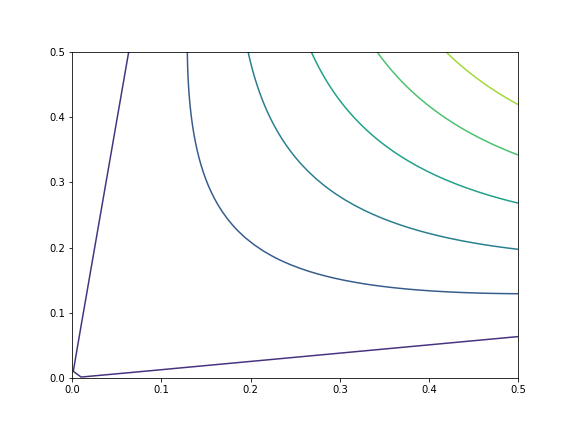
\includegraphics[width=\textwidth]{q9.png}
				\caption{Plot of the corner response function}
			\end{figure}
		
		\item[b] \mbox{}\\
			\begin{lstlisting}[language=Python, caption=Implementation of function $Q_a$]
				def getHarrisCornerResponse(I, h, alpha, threshold=0.8):
					    '''
					    This function calculate the Harris corner response funciton
					    
					    Inputs:
					    * I: 2*2 array of Image with grey levels
					    * h: filter, uniform, gaussian, etc.
					    * alpha: parameter of the corner response equation
					    * threshold: if <1, apply threshold based on the maximum of corner response value, otherwise, directly apply input value
					    
					    Outputs:
					    * Q: Matrix container response value
					    * coordinates: 
					        tuple contains two arrays, 
					            first array is the x coordiate of the potins has corner response value larger than threshold
					            second array is the y coordiate of the potins has corner response value larger than threshold
					    '''
					    (M,N) = I.shape
					    hx = np.array([[0,0.5,0],[0,0,0],[0,-0.5,0]])
					    Ix = scipy.ndimage.filters.convolve(I,hx)
					    Ix2 = np.power(Ix, 2)
					    hy = hx.transpose()
					    Iy = scipy.ndimage.filters.convolve(I,hy)
					    Iy2 = np.power(Iy, 2)
					    IxIy =  scipy.ndimage.filters.convolve(Ix,hy)
					    ul =  scipy.ndimage.filters.convolve(Ix2,h)
					    ur =  scipy.ndimage.filters.convolve(IxIy,h)
					    bl =  scipy.ndimage.filters.convolve(IxIy,h)
					    br = scipy.ndimage.filters.convolve(Iy2,h)
					    Q_alpha = np.zeros((M,N))
					    for i_ind in range(M):
					        for j_ind in range(N):
					            m_bar = np.array([[ul[i_ind,j_ind], ur[i_ind,j_ind]],[bl[i_ind,j_ind],br[i_ind,j_ind]]])
					            Q_alpha[i_ind,j_ind] = np.linalg.det(m_bar) - alpha*(np.trace(m_bar))**2
					    if threshold<=1:
					        t = np.max(Q_alpha)*threshold
					    else:
					        t= threshold
					    coordinates = np.where(Q_alpha>t)
					    return Q_alpha, coordinates
			\end{lstlisting}
			
			\begin{lstlisting}[language=Python, caption=house with uniform filter]
				n = 3
				w = np.ones(shape=(n,n))
				h = w
				Q,coordinates = getHarrisCornerResponse(I,h,0.05, 0.03)
				fig=plt.figure(1,figsize=(M/20,N/20))
				plt.imshow(I,cmap=cm.gray,vmin=0,vmax=255)
				plt.scatter(coordinates[1],coordinates[0],c='r', s=5)
				plt.axis('off')
				fig.savefig('q9_house_uniform_filter.png', dpi=fig.dpi)
			\end{lstlisting}
			
			\begin{figure}[h]
				\centering
				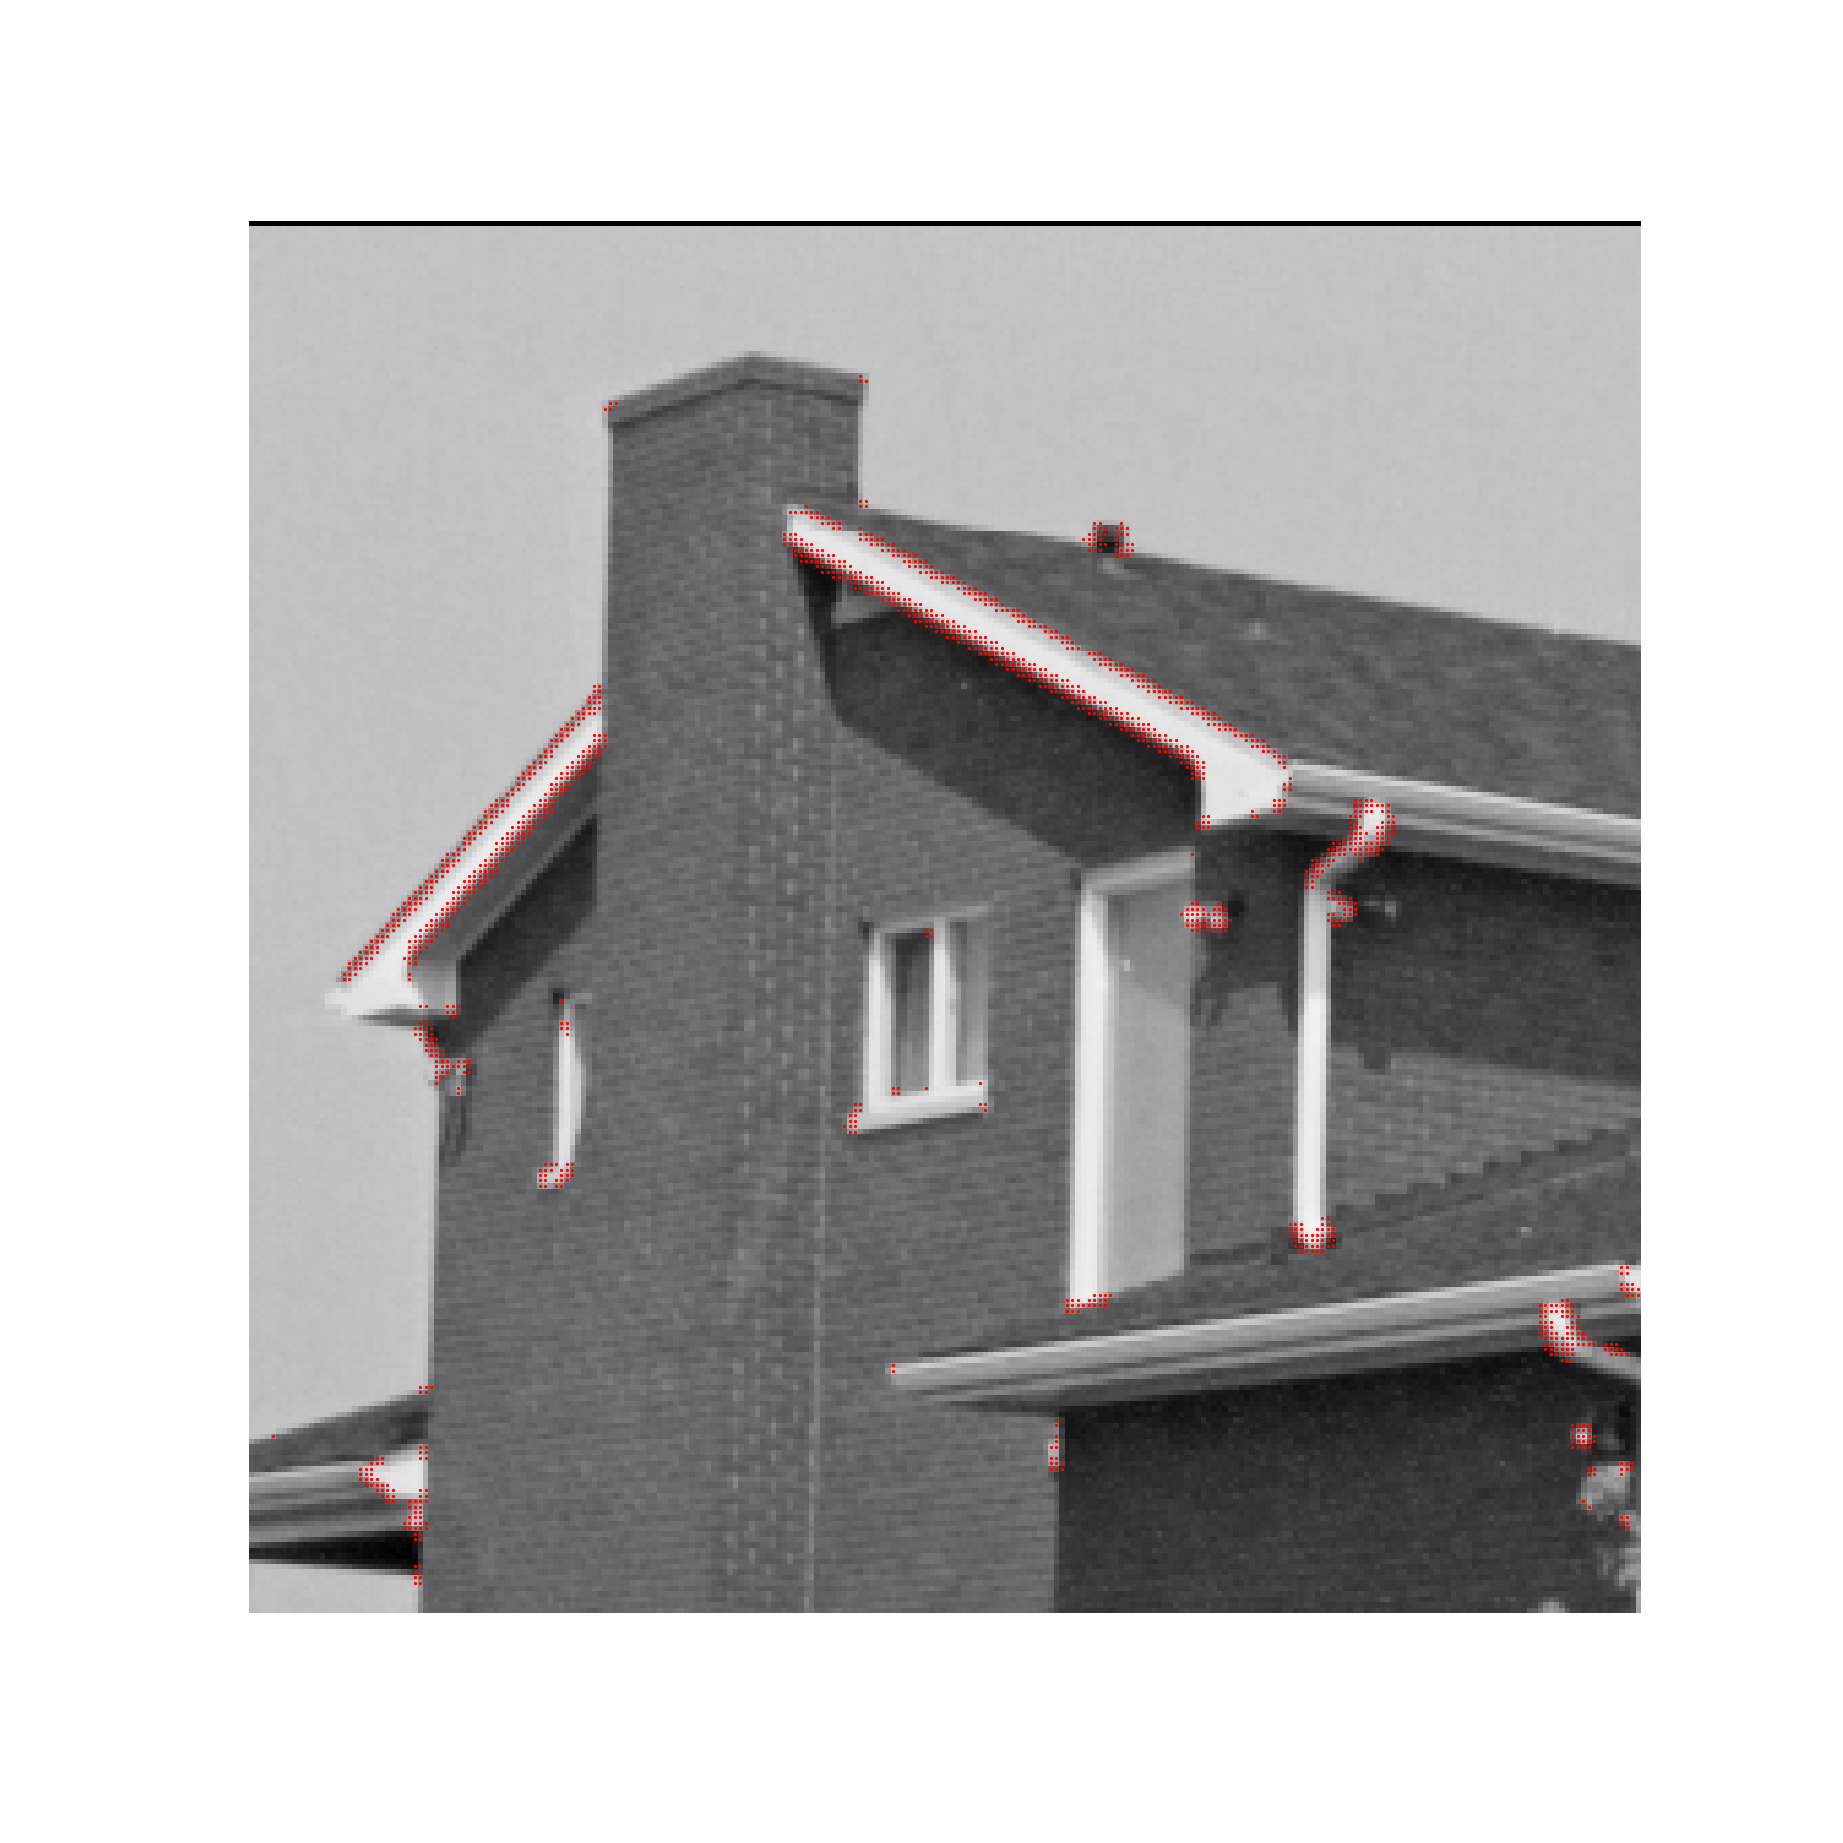
\includegraphics[width=\textwidth]{q9_house_uniform_filter.png}
				\caption{house with uniform filter}
			\end{figure}
			
			\begin{lstlisting}[language=Python, caption=house with gaussian filter]
				def gaussian(x,y,sigma):
				    return exp(-(x**2+y**2)/(2*sigma**2))
				n = 5
				sigma=1
				_hG = np.array([[ gaussian(r, c, sigma) for c in range(int(-(n-1)/2),int((n-1)/2 + 1))] 
				                for r in range(int(-(n-1)/2),int((n-1)/2 + 1))])
				hG = _hG/np.sum(_hG)
				Q,coordinates = getHarrisCornerResponse(I,hG,0.05, 0.01)
				fig=plt.figure(1,figsize=(M/20,N/20))
				plt.imshow(I,cmap=cm.gray,vmin=0,vmax=255)
				plt.scatter(coordinates[1],coordinates[0],c='r', s=5)
				plt.axis('off')
				fig.savefig('q9_house_gaussian_filter.png', dpi=fig.dpi)
			\end{lstlisting}
			
			\begin{figure}[h]
				\centering
				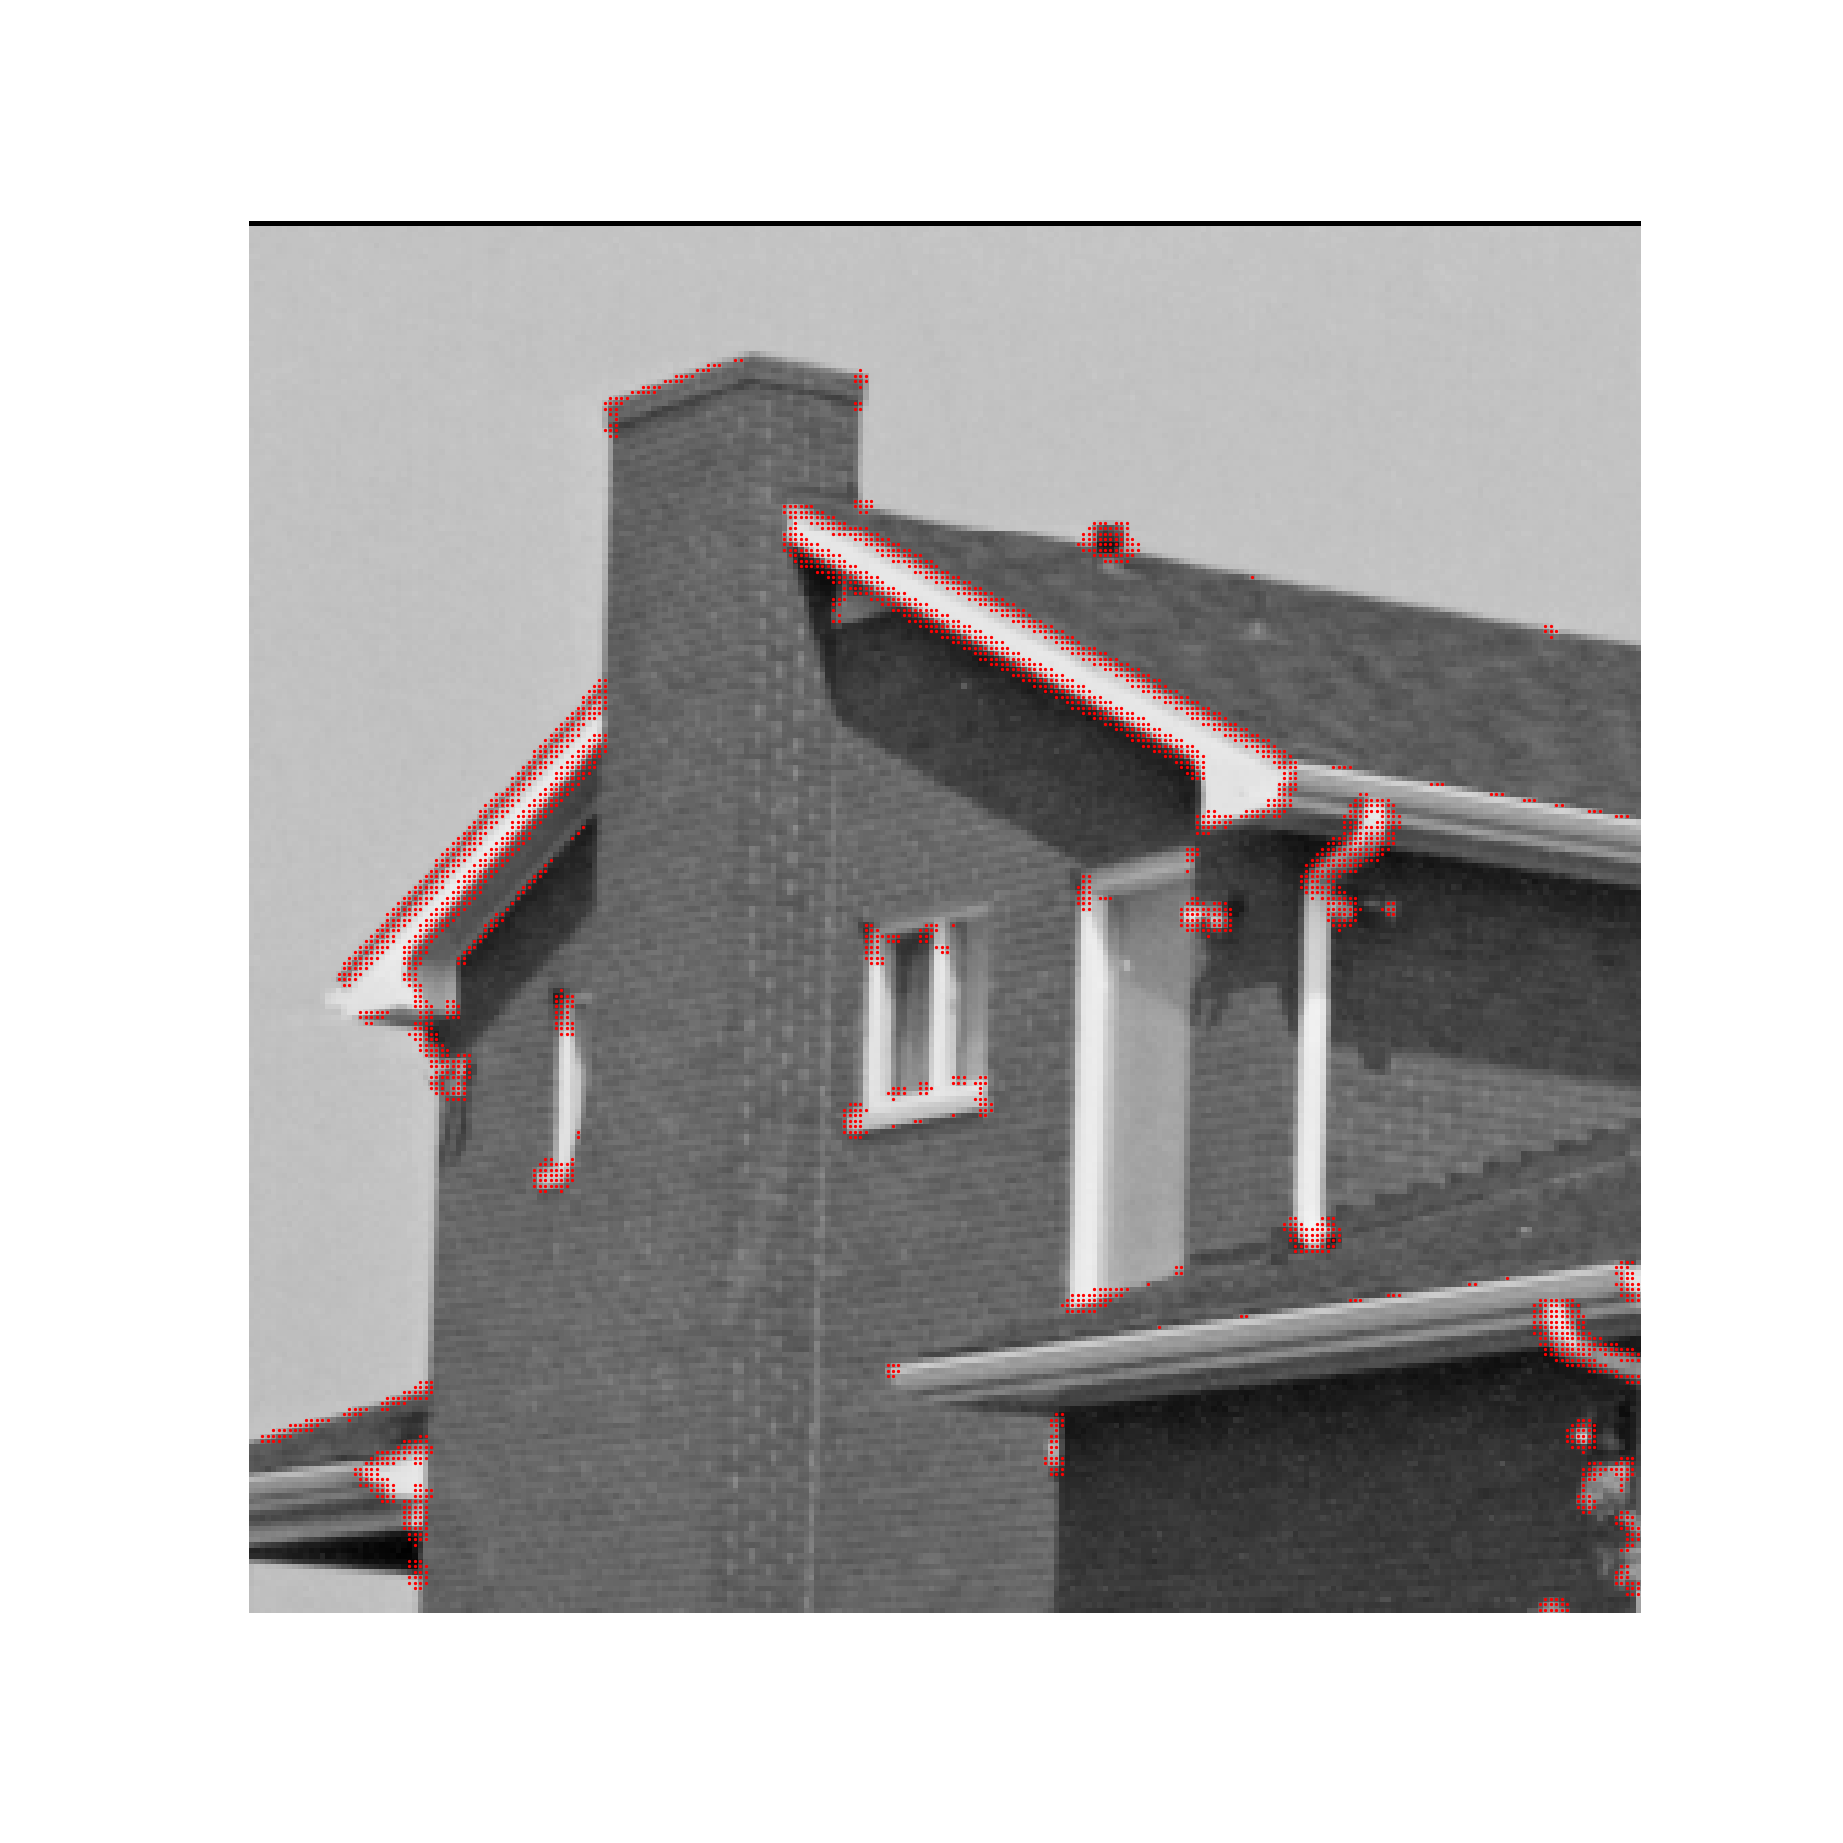
\includegraphics[width=\textwidth]{q9_house_gaussian_filter.png}
				\caption{house with gaussian filter}
			\end{figure}
			
			\begin{lstlisting}[language=Python, caption=polygon with uniform filter]
				n = 3
				w = np.ones(shape=(n,n))
				h = w
				Q,coordinates = getHarrisCornerResponse(I,h,0.05, 1e7)
				fig=plt.figure(1,figsize=(M/20,N/20))
				plt.imshow(I,cmap=cm.gray,vmin=0,vmax=255)
				plt.scatter(coordinates[1],coordinates[0],c='r', s=5)
				plt.axis('off')
				fig.savefig('q9_polygons_uniform_filter.png', dpi=fig.dpi)
			\end{lstlisting}
			
			\begin{figure}[h]
				\centering
				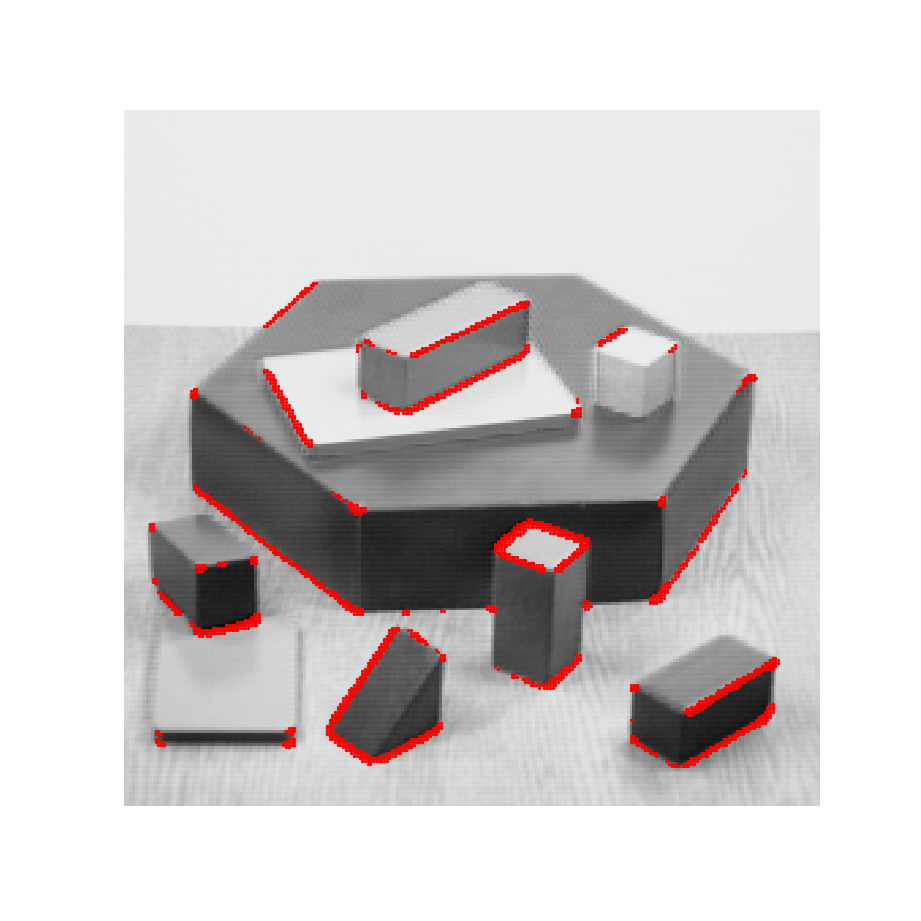
\includegraphics[width=\textwidth]{q9_polygons_uniform_filter.png}
				\caption{polygon with uniform filter}
			\end{figure}
			
			\begin{lstlisting}[language=Python, caption=polygon with gaussian filter]
				n = 5
				sigma=1
				_hG = np.array([[ gaussian(r, c, sigma) for c in range(int(-(n-1)/2),int((n-1)/2 + 1))] 
				                for r in range(int(-(n-1)/2),int((n-1)/2 + 1))])
				hG = _hG/np.sum(_hG)
				Q,coordinates = getHarrisCornerResponse(I,hG,0.05, 0.1)
				fig=plt.figure(1,figsize=(M/20,N/20))
				plt.imshow(I,cmap=cm.gray,vmin=0,vmax=255)
				plt.scatter(coordinates[1],coordinates[0],c='r', s=5)
				plt.axis('off')
				fig.savefig('q9_polygons_gaussian_filter.png', dpi=fig.dpi)
			\end{lstlisting}
			
			\begin{figure}[h]
				\centering
				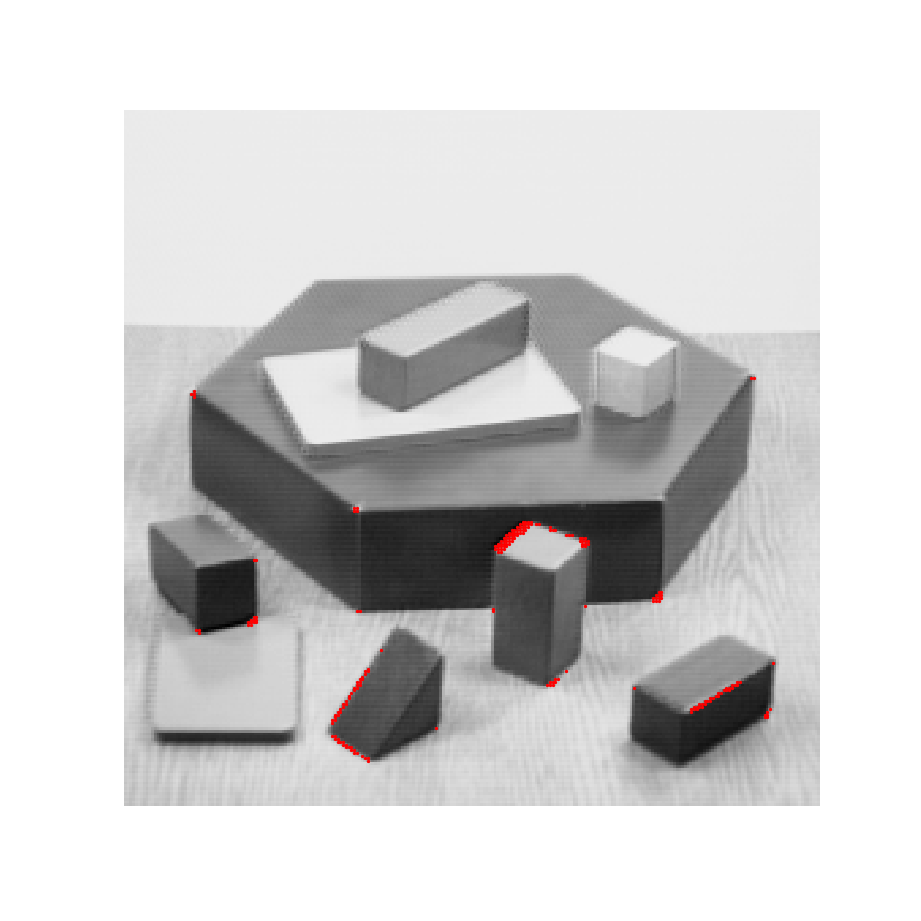
\includegraphics[width=\textwidth]{q9_polygons_gaussian_filter.png}
				\caption{polygon with gaussian filter}
			\end{figure}
			
			\begin{lstlisting}[language=Python, caption=grand mosque with uniform filter]
				n = 3
				w = np.ones(shape=(n,n))
				h = w
				Q,coordinates = getHarrisCornerResponse(I,h,0.05, 0.05)
				fig=plt.figure(1,figsize=(M/20,N/20))
				plt.imshow(I,cmap=cm.gray,vmin=0,vmax=255)
				plt.scatter(coordinates[1],coordinates[0],c='r', s=5)
				plt.axis('off')
				fig.savefig('q9_uae_uniform_filter.png', dpi=fig.dpi)
			\end{lstlisting}
			
			\begin{figure}[h]
				\centering
				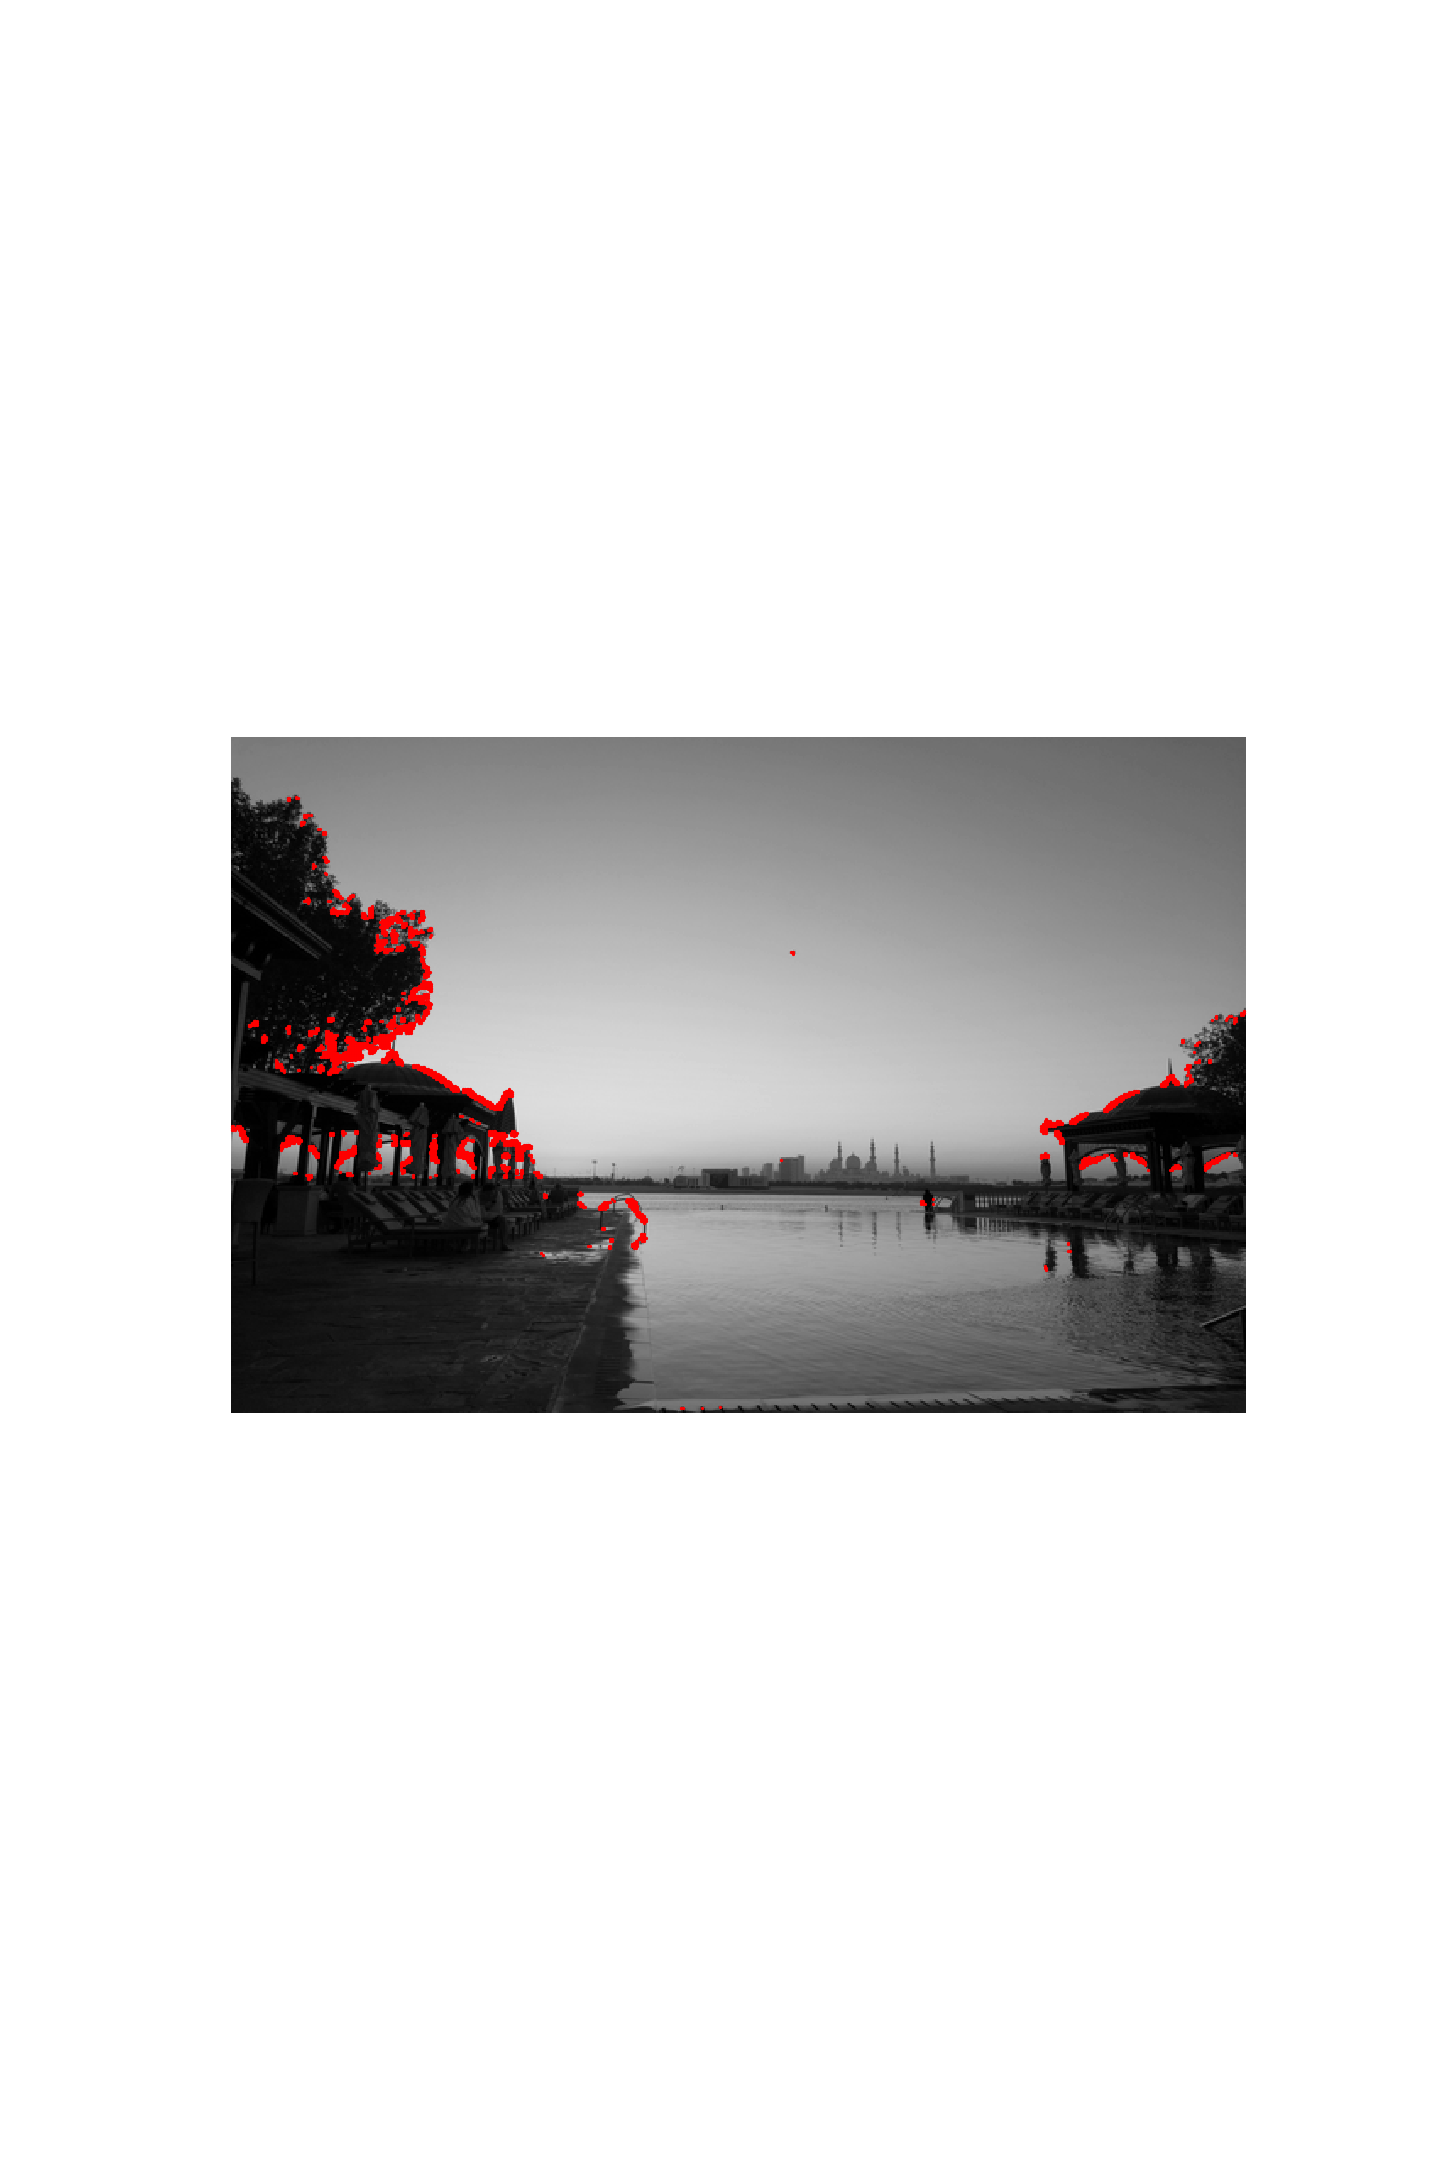
\includegraphics[width=\textwidth]{q9_uae_uniform_filter.png}
				\caption{grand mosque with uniform filter}
			\end{figure}
			
			\begin{lstlisting}[language=Python, caption=grand mosque with gaussian filter]
				n = 5
				sigma=1
				_hG = np.array([[ gaussian(r, c, sigma) for c in range(int(-(n-1)/2),int((n-1)/2 + 1))] 
				                for r in range(int(-(n-1)/2),int((n-1)/2 + 1))])
				hG = _hG/np.sum(_hG)
				Q,coordinates = getHarrisCornerResponse(I,hG,0.05, 0.1)
				fig=plt.figure(1,figsize=(M/20,N/20))
				plt.imshow(I,cmap=cm.gray,vmin=0,vmax=255)
				plt.scatter(coordinates[1],coordinates[0],c='r', s=5)
				plt.axis('off')
				fig.savefig('q9_uae_gaussian_filter.png', dpi=fig.dpi)
			\end{lstlisting}
			
			\begin{figure}[h]
				\centering
				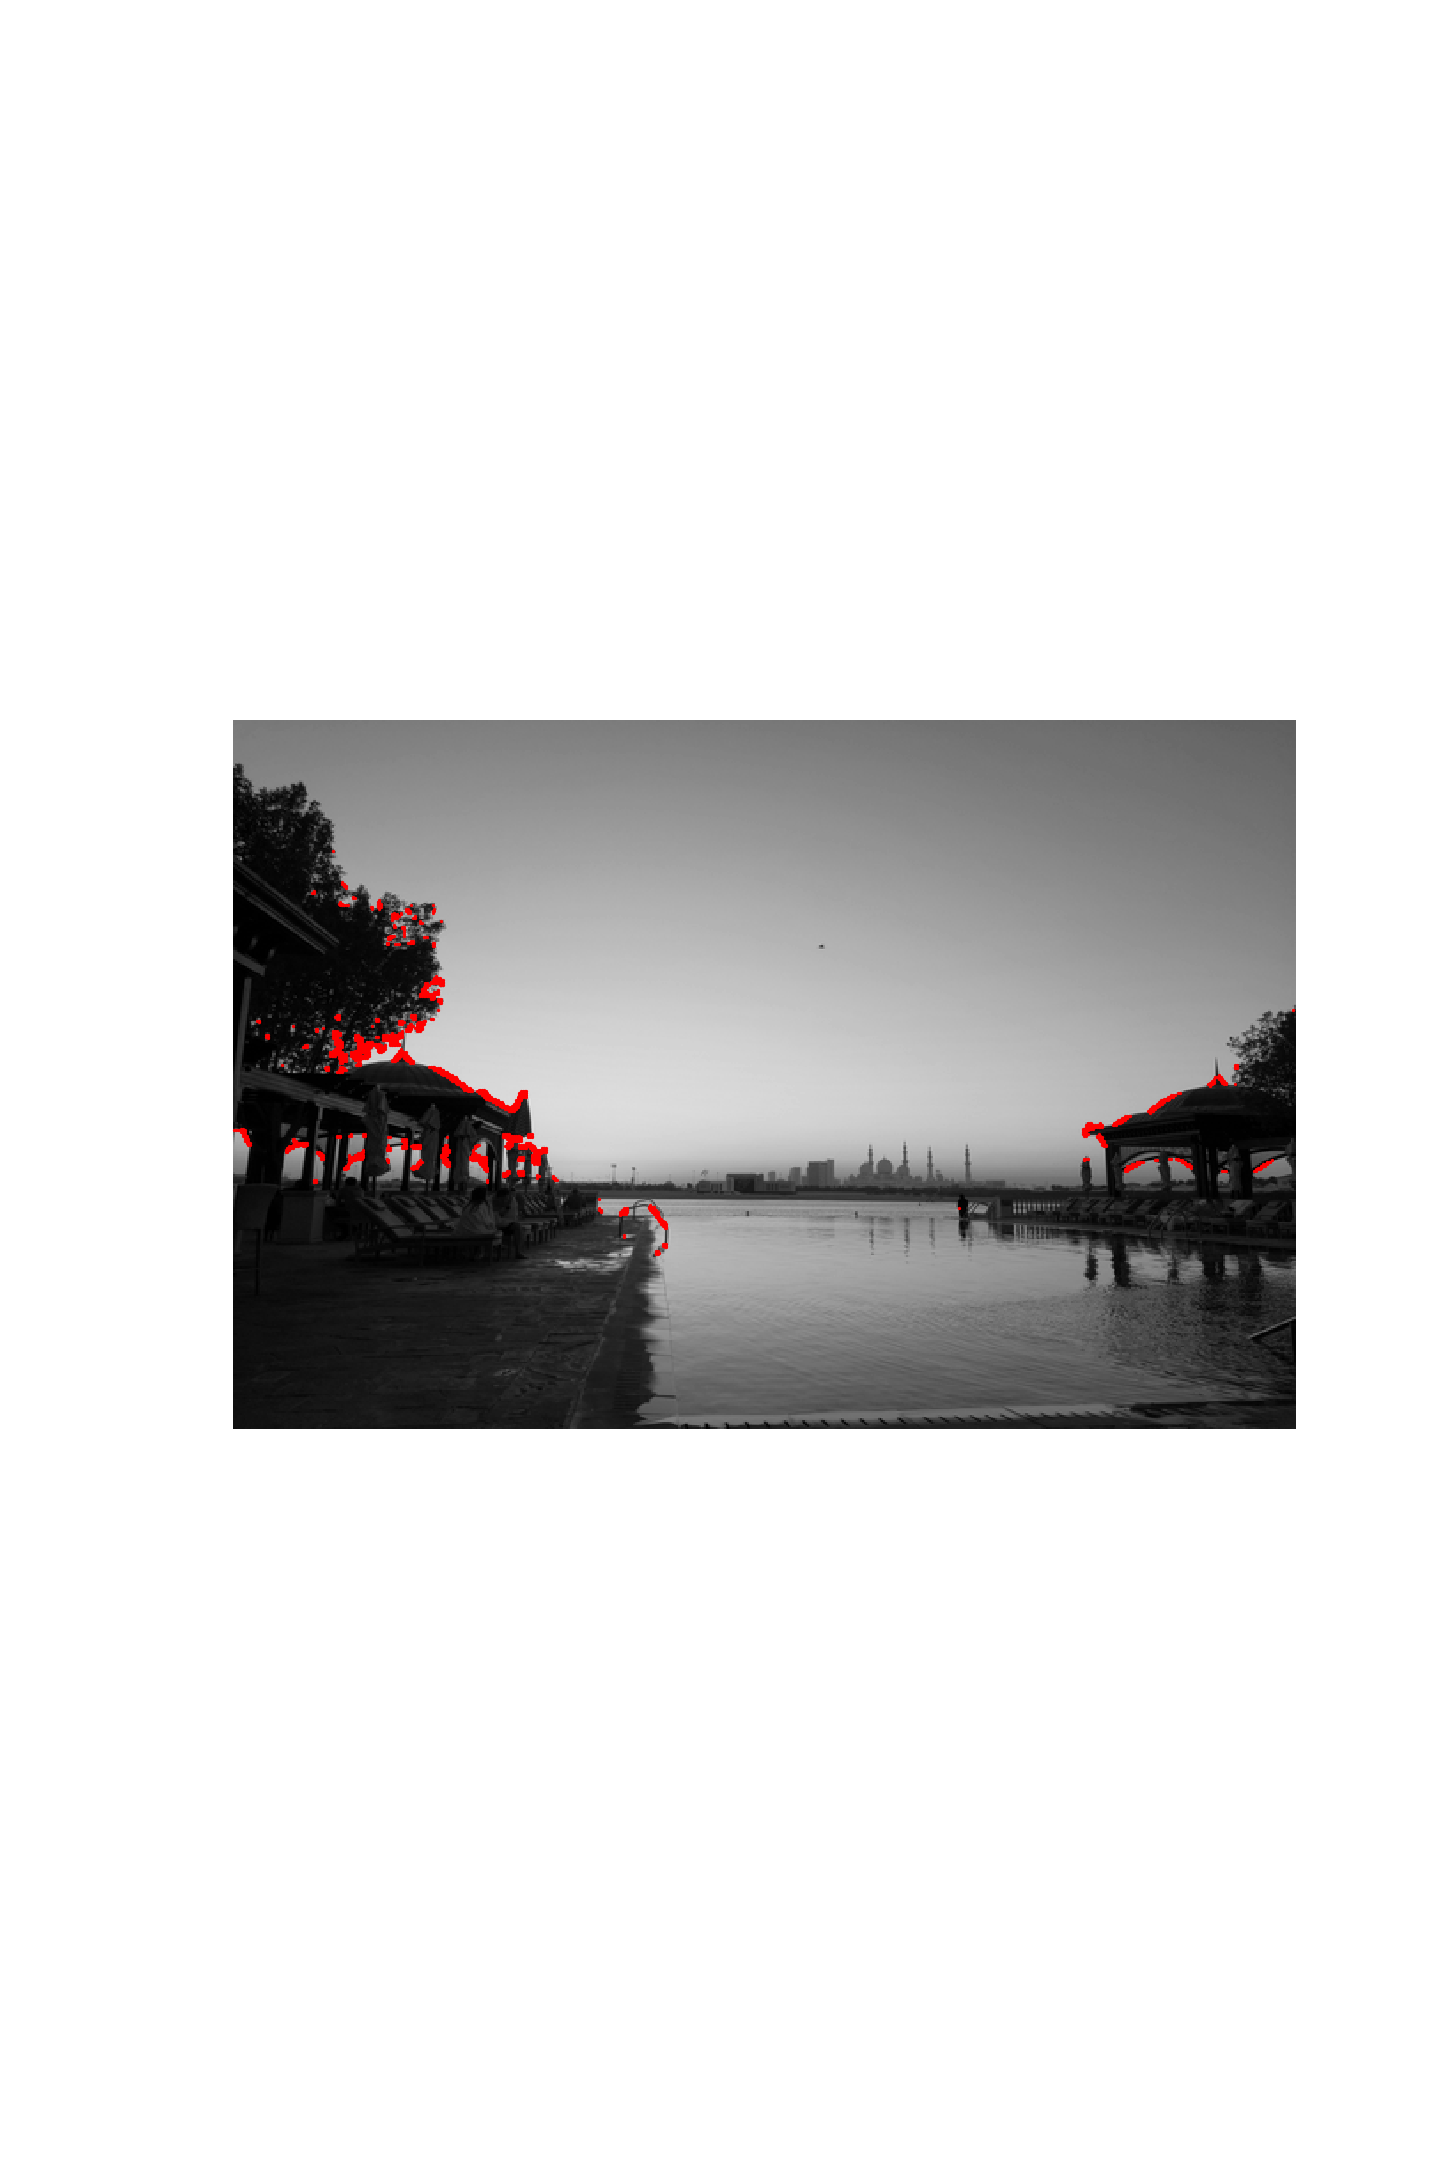
\includegraphics[width=\textwidth]{q9_uae_gaussian_filter.png}
				\caption{grand mosque with gaussian filter}
			\end{figure}
			
	\end{enumerate}

\end{solution}


\end{document}












